\chapter{Printing and Assembly}
\label{ch:printingandassembly}

In this chapter, the process of printing and assembling the prototype is described.

\section{Printing}
\label{sec:printing}

In this section, the process of printing the prototype is described. The prototype was printed using the Prusa Slicer i3 MK3S+ 3D printer. The printing process was performed in the Workshop of the University of Applied Sciences Brandenburg. The printing process was performed using the following parameters:

\begin{itemize}
    \item Layer Height: 0.2 mm
    \item Infill Density: 15\%
    \item Print Speed: 60 mm/s
    \item Supports: Yes
    \item Filament: PLA
\end{itemize}

The printing process was performed using the PrusaSlicer software. The PrusaSlicer software was used to generate the G-code for the printing process. Table \ref{tab:finalprintingtimeandfilament} shows the printing time and the amount of filament used for the printing process. The printed parts with its support materials removed are shown in Figure \ref{fig:printedparts}.


\begin{table}[!ht]
    \centering
    \begin{tabular}{|l|l|l|}
        \hline
        \textbf{Part Name} & \textbf{Mass of PLA used (g)} & \textbf{Printing Time (h)} \\ \hline
        Top Cover          & 57.71                         & 2.00                       \\ \hline
        Main Body          & 245.05                        & 9.23                       \\ \hline
        Battery Cover      & 22.21                         & 0.67                       \\ \hline
        Switch Cover       & 1.31                          & 0.05                       \\ \hline
        Handle Pistol      & 64.63                         & 1.98                       \\ \hline
        Total              & 390.91                        & 13.93                      \\ \hline
    \end{tabular}
    \caption{Printing Time and Filament Used}
    \label{tab:finalprintingtimeandfilament}
\end{table}



\begin{figure}[h!]
    \centering
    \begin{subfigure}[c]{0.45\textwidth}
        \begin{minipage}{\textwidth}
            \centering
            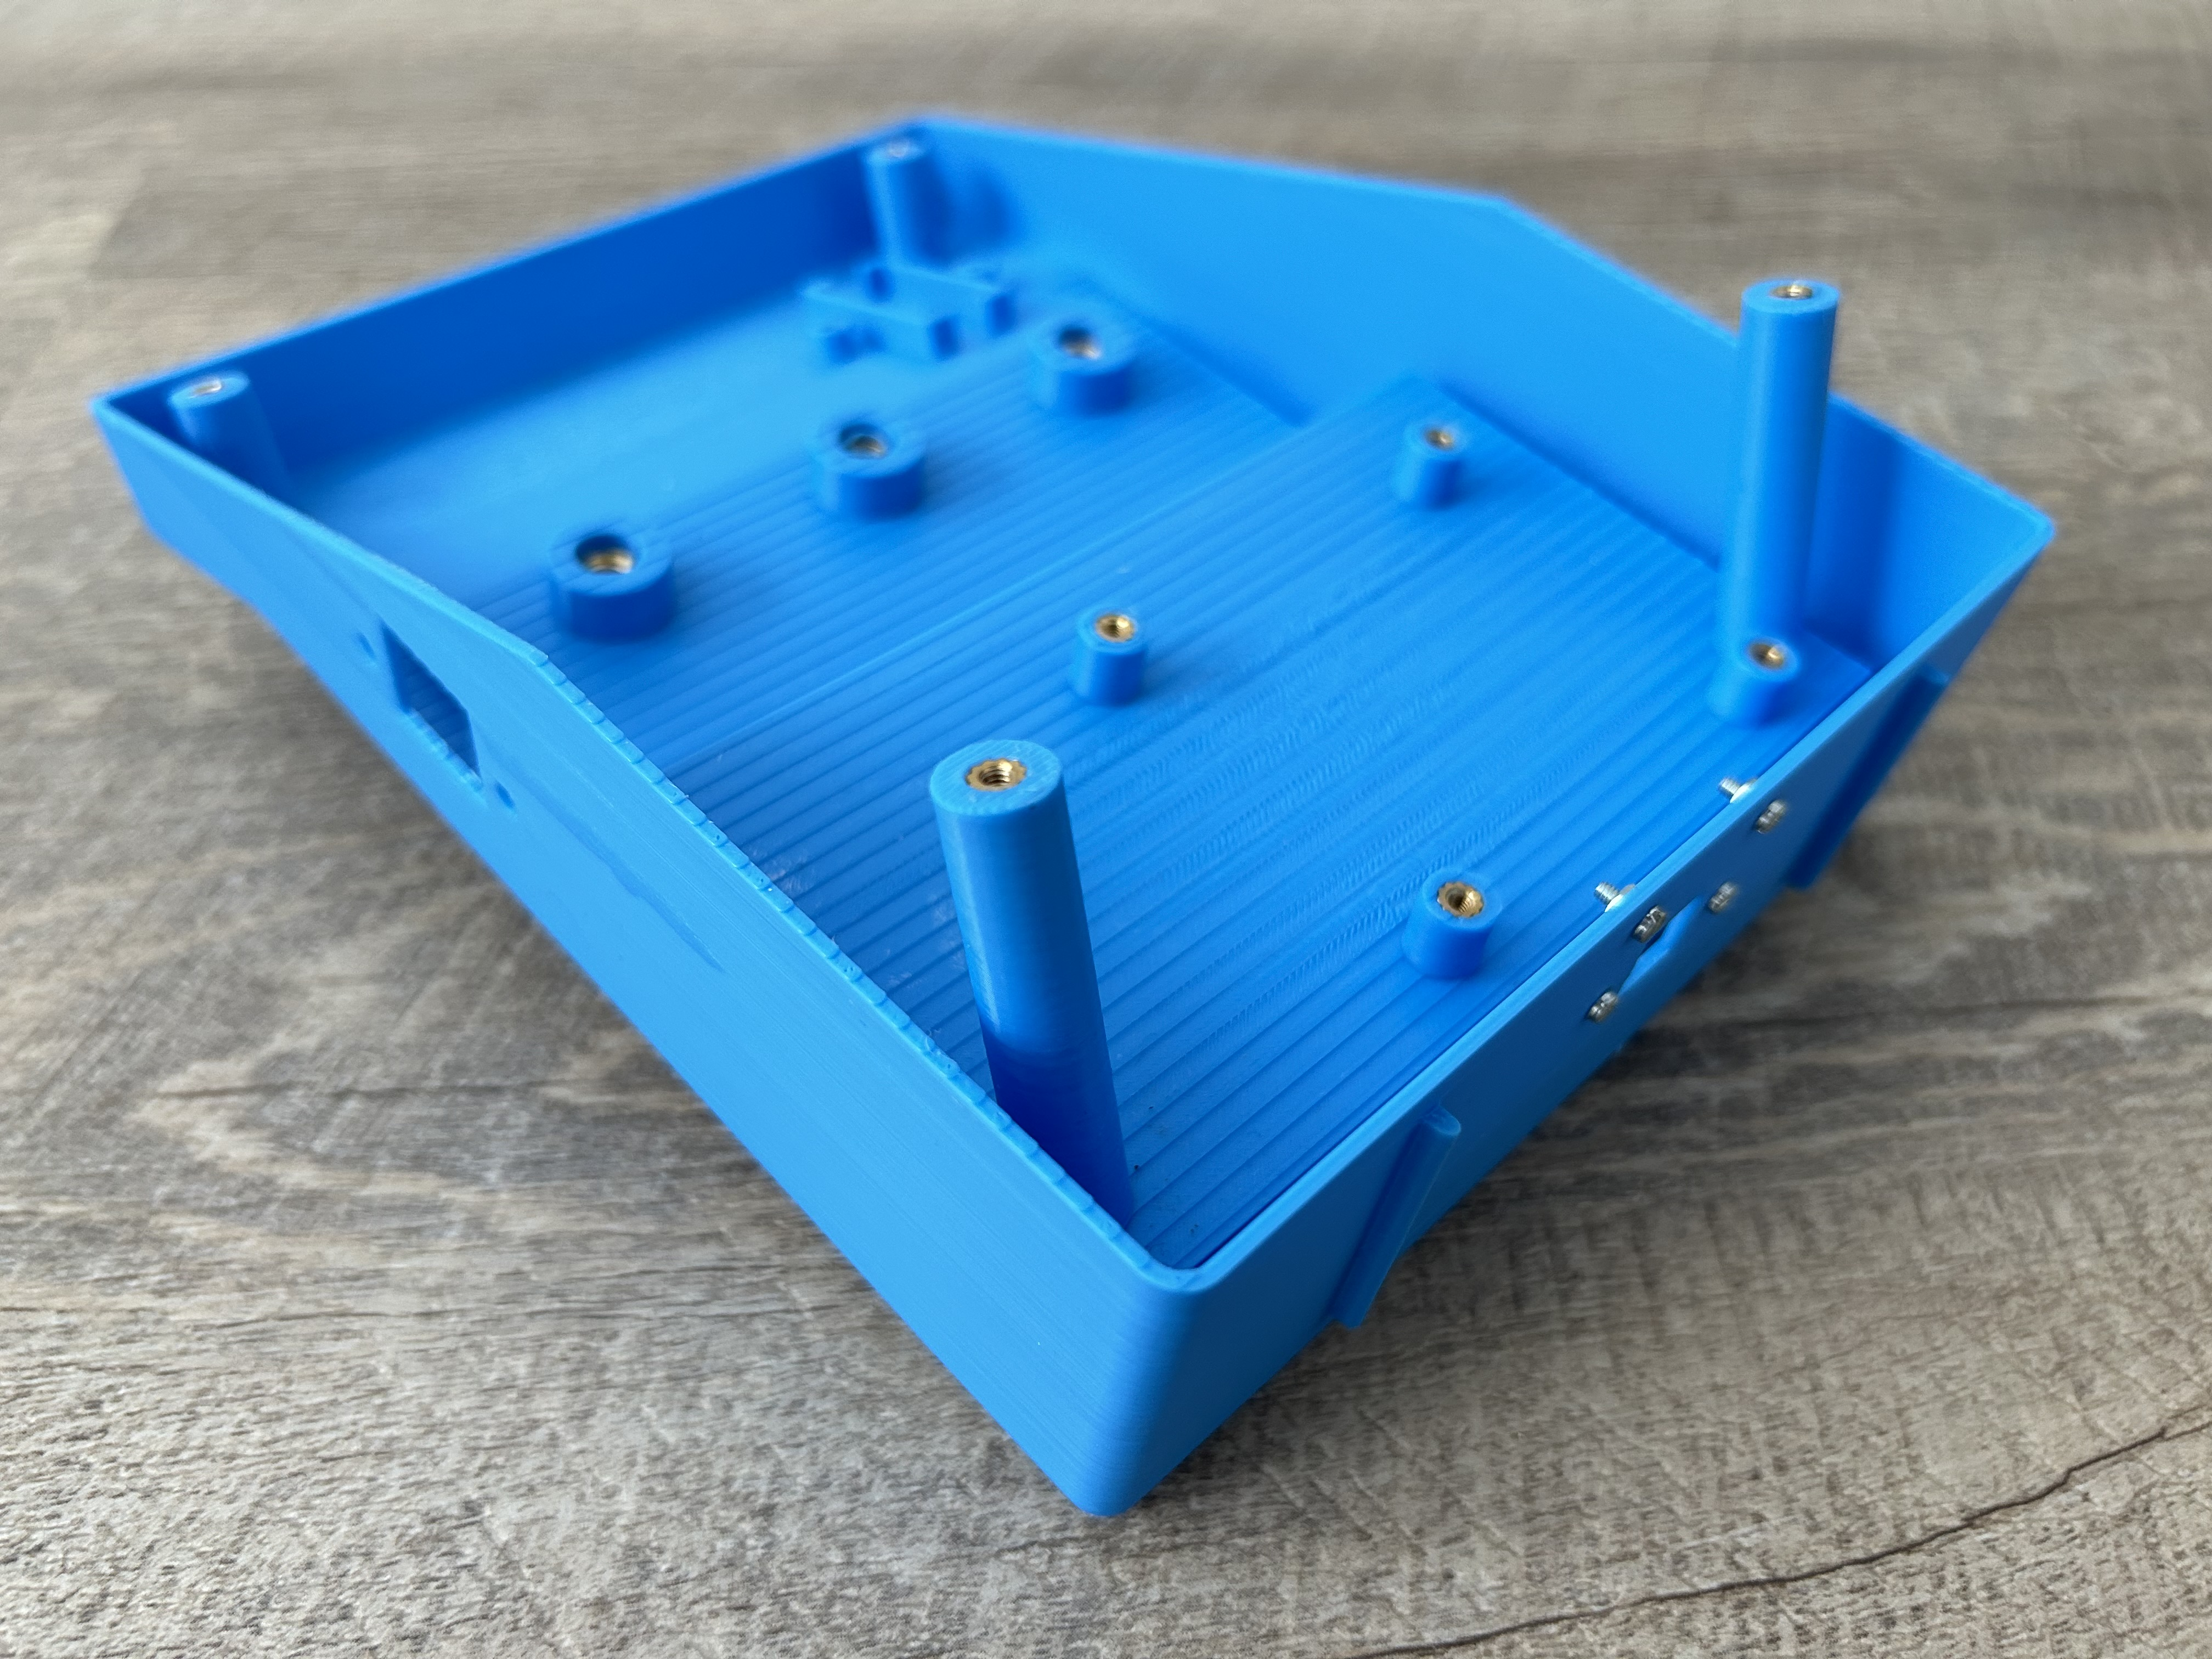
\includegraphics[height=4 cm]{texs/Part1/chapter5/image/res_main.jpg}
        \end{minipage}
        \caption{Main Body}
        \label{fig:printed_main_body}
    \end{subfigure}
    \begin{subfigure}[c]{0.45\textwidth}
        \begin{minipage}{\textwidth}
            \centering
            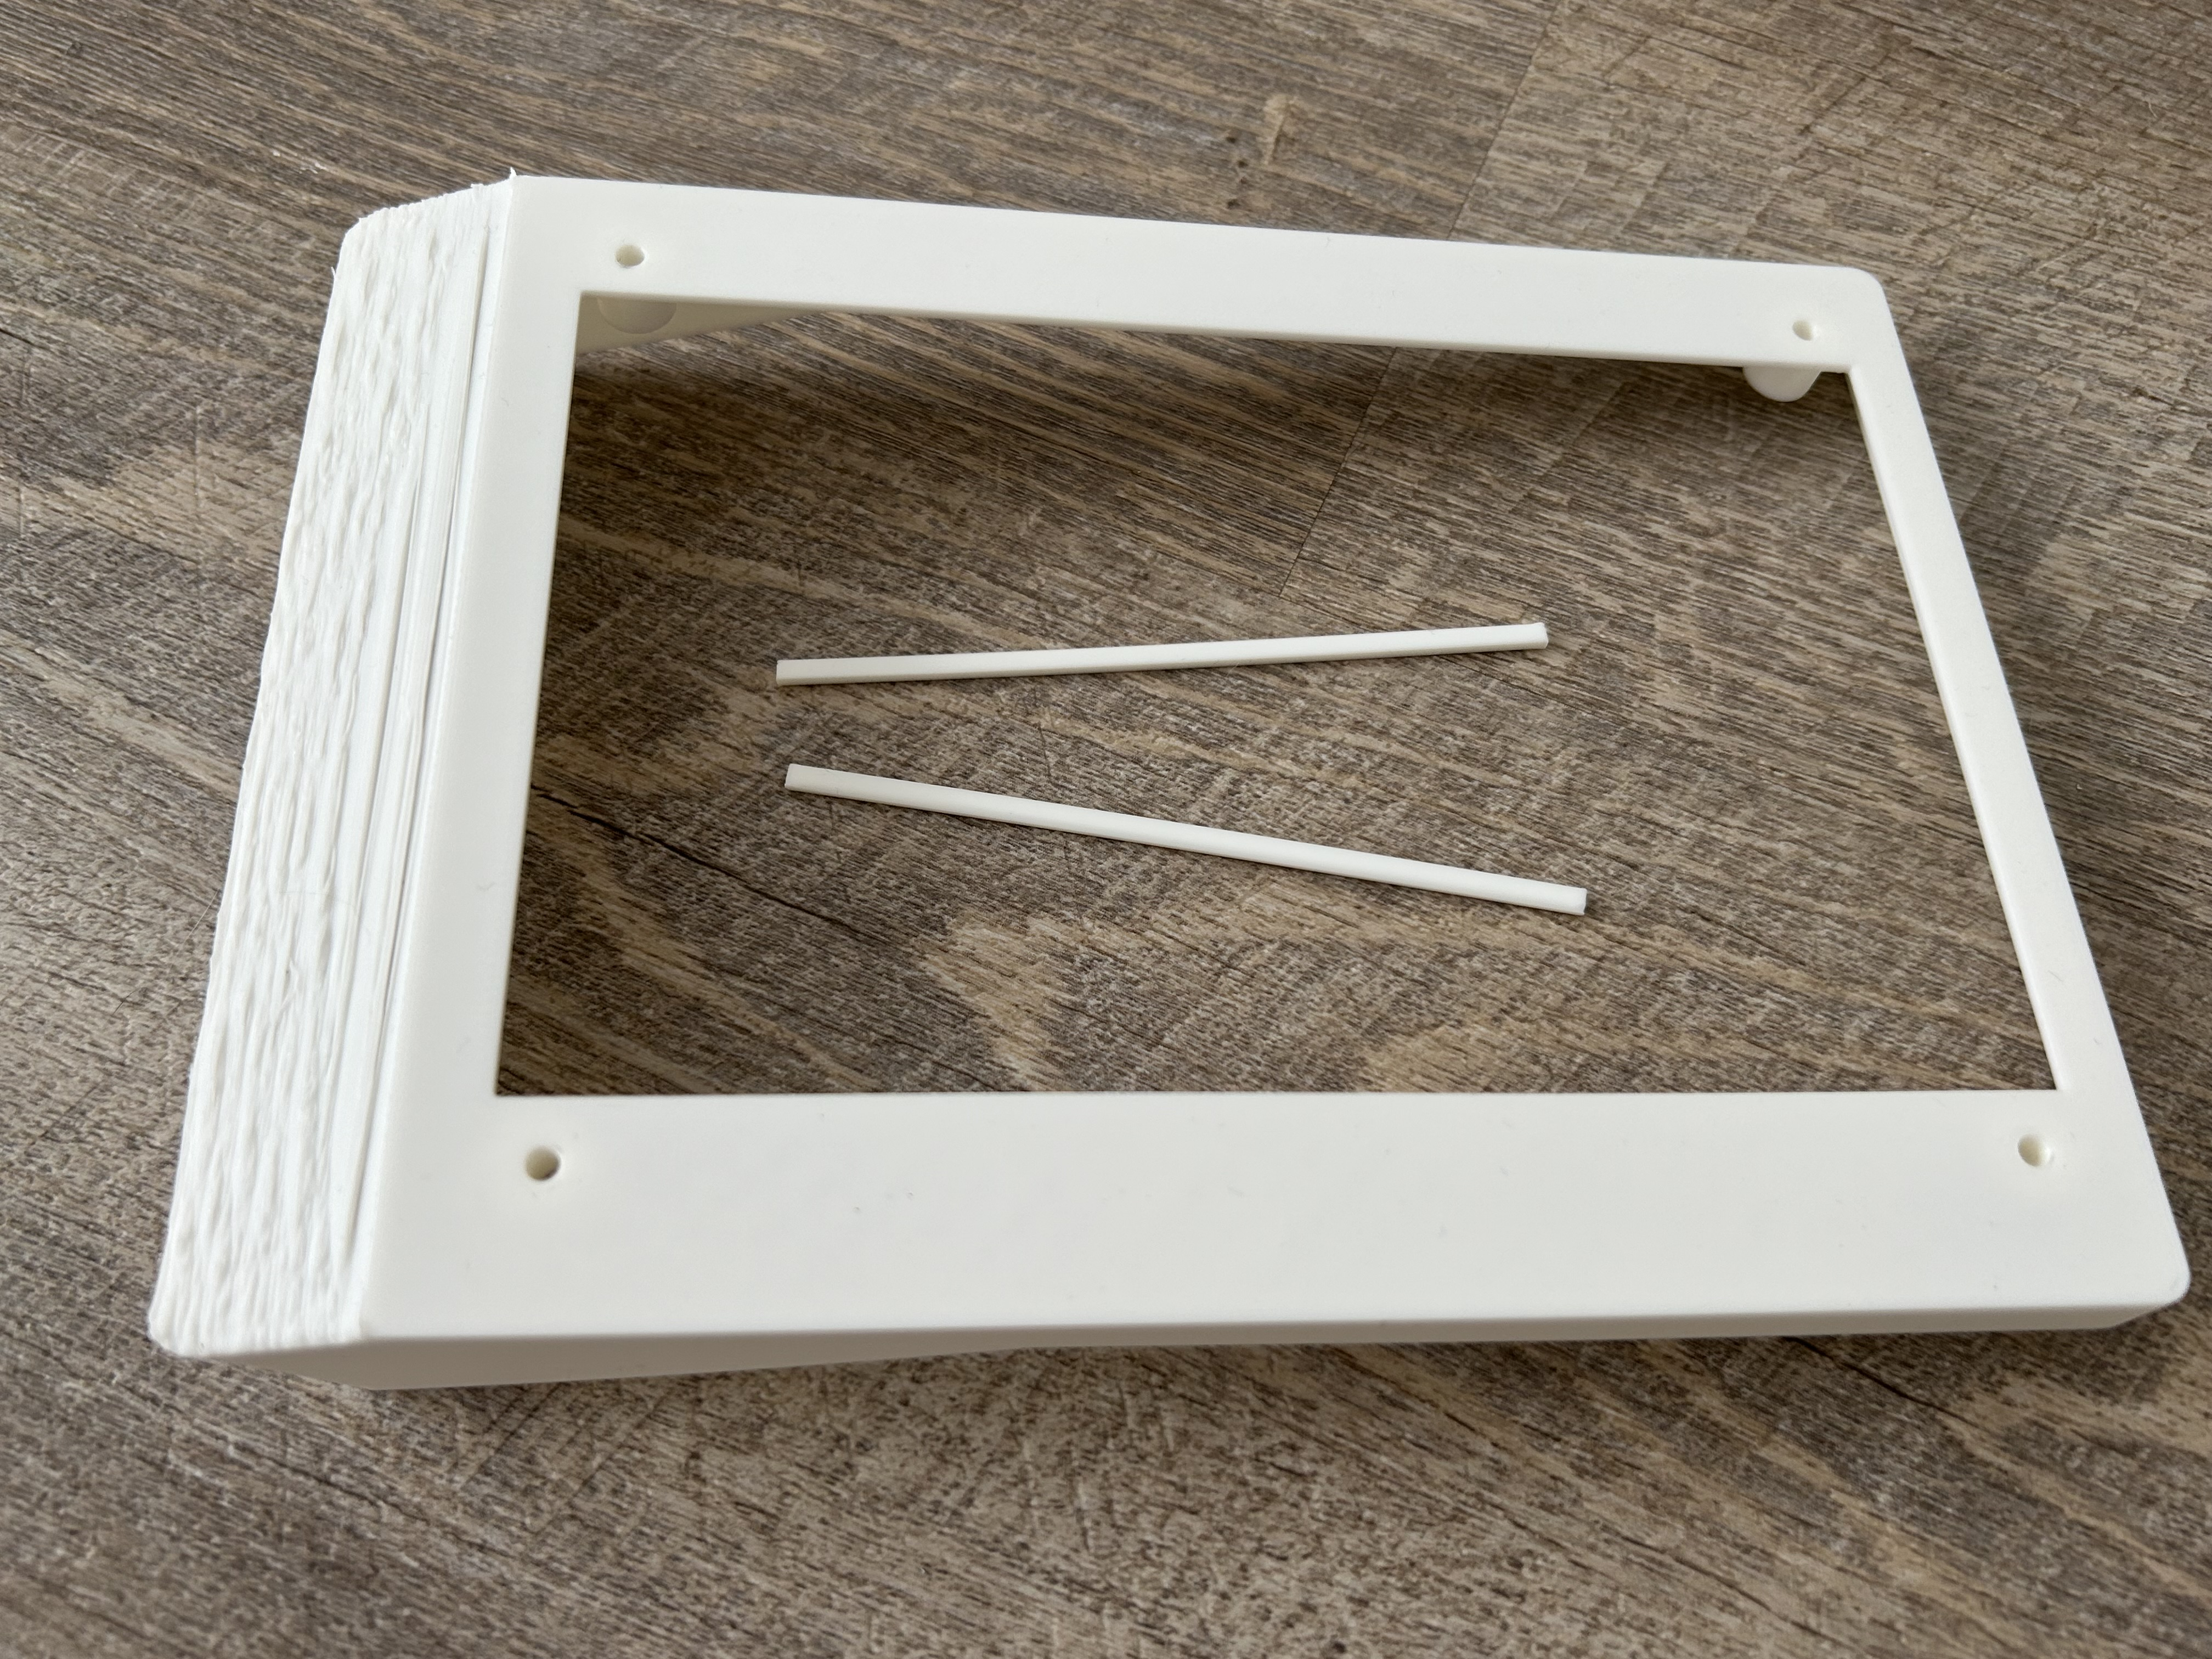
\includegraphics[height=4 cm]{texs/Part1/chapter5/image/res_top.jpg}
        \end{minipage}
        \caption{Top Cover}
        \label{fig:printed_top_cover}
    \end{subfigure}
    \begin{subfigure}[c]{0.45\textwidth}
        \begin{minipage}{\textwidth}
            \centering
            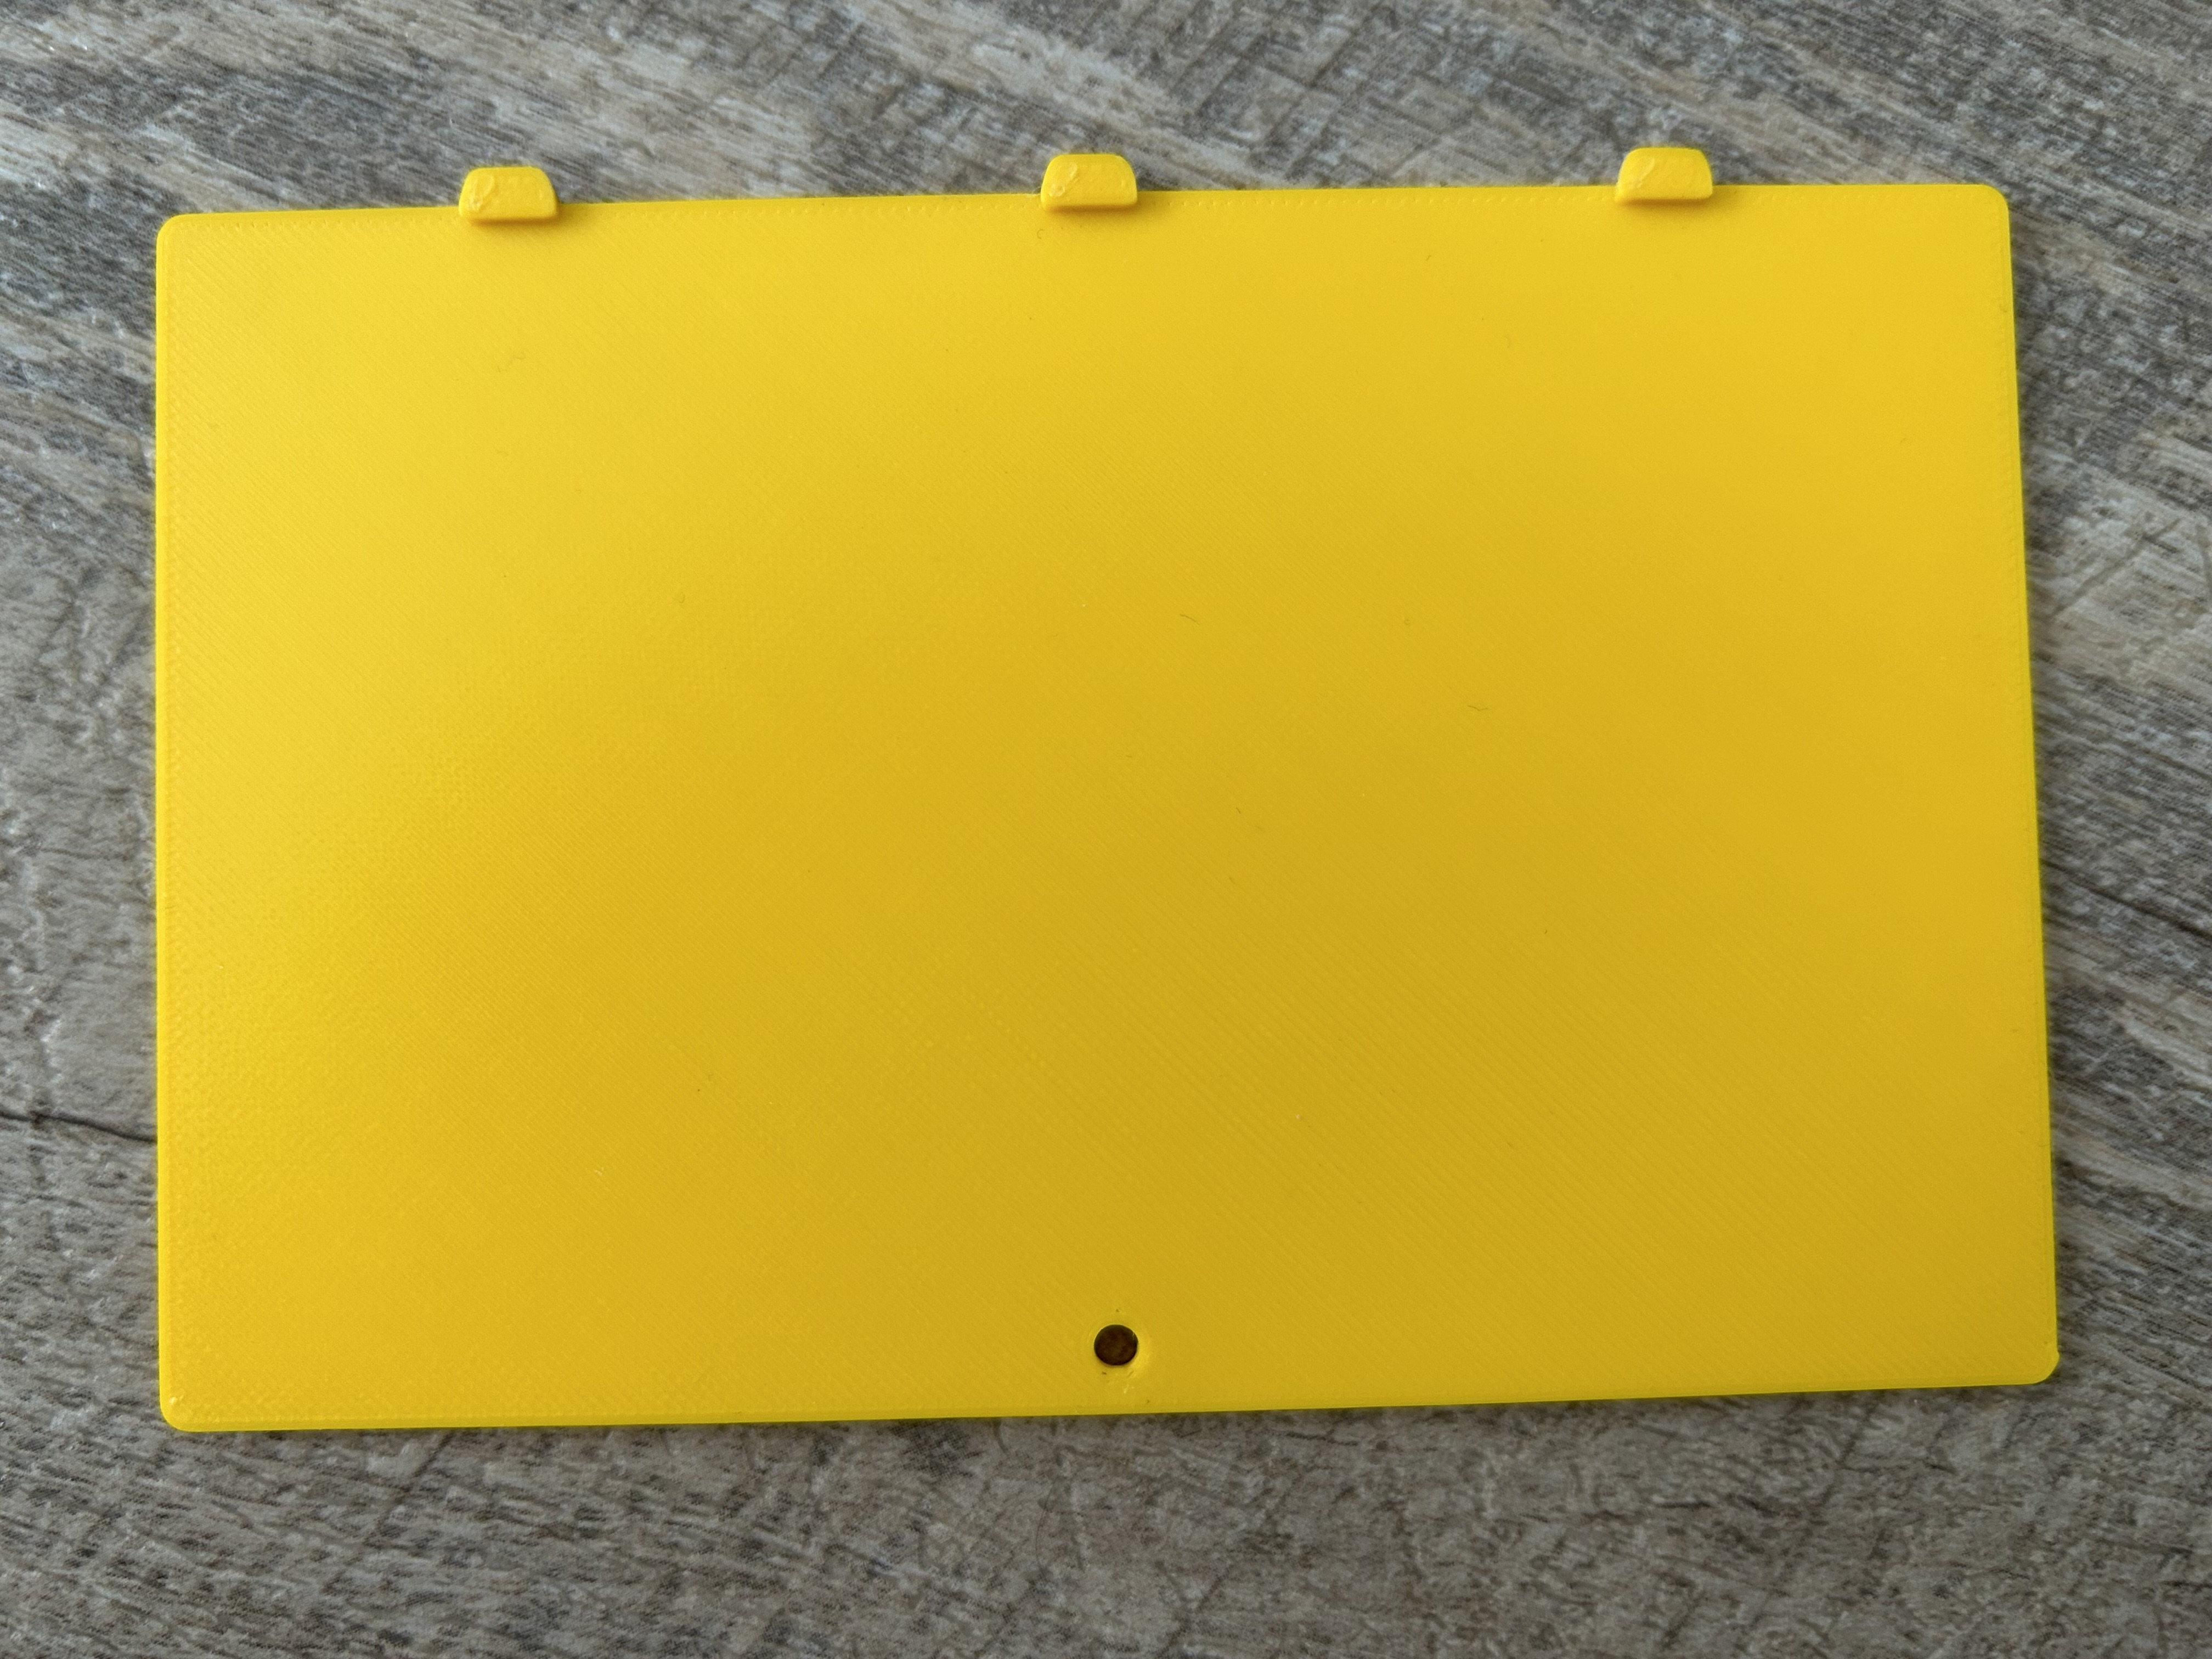
\includegraphics[height=4 cm]{texs/Part1/chapter5/image/res_batt.jpg}
        \end{minipage}
        \caption{Battery Cover}
        \label{fig:printed_battery_cover}
    \end{subfigure}
    \begin{subfigure}[c]{0.45\textwidth}
        \begin{minipage}{\textwidth}
            \centering
            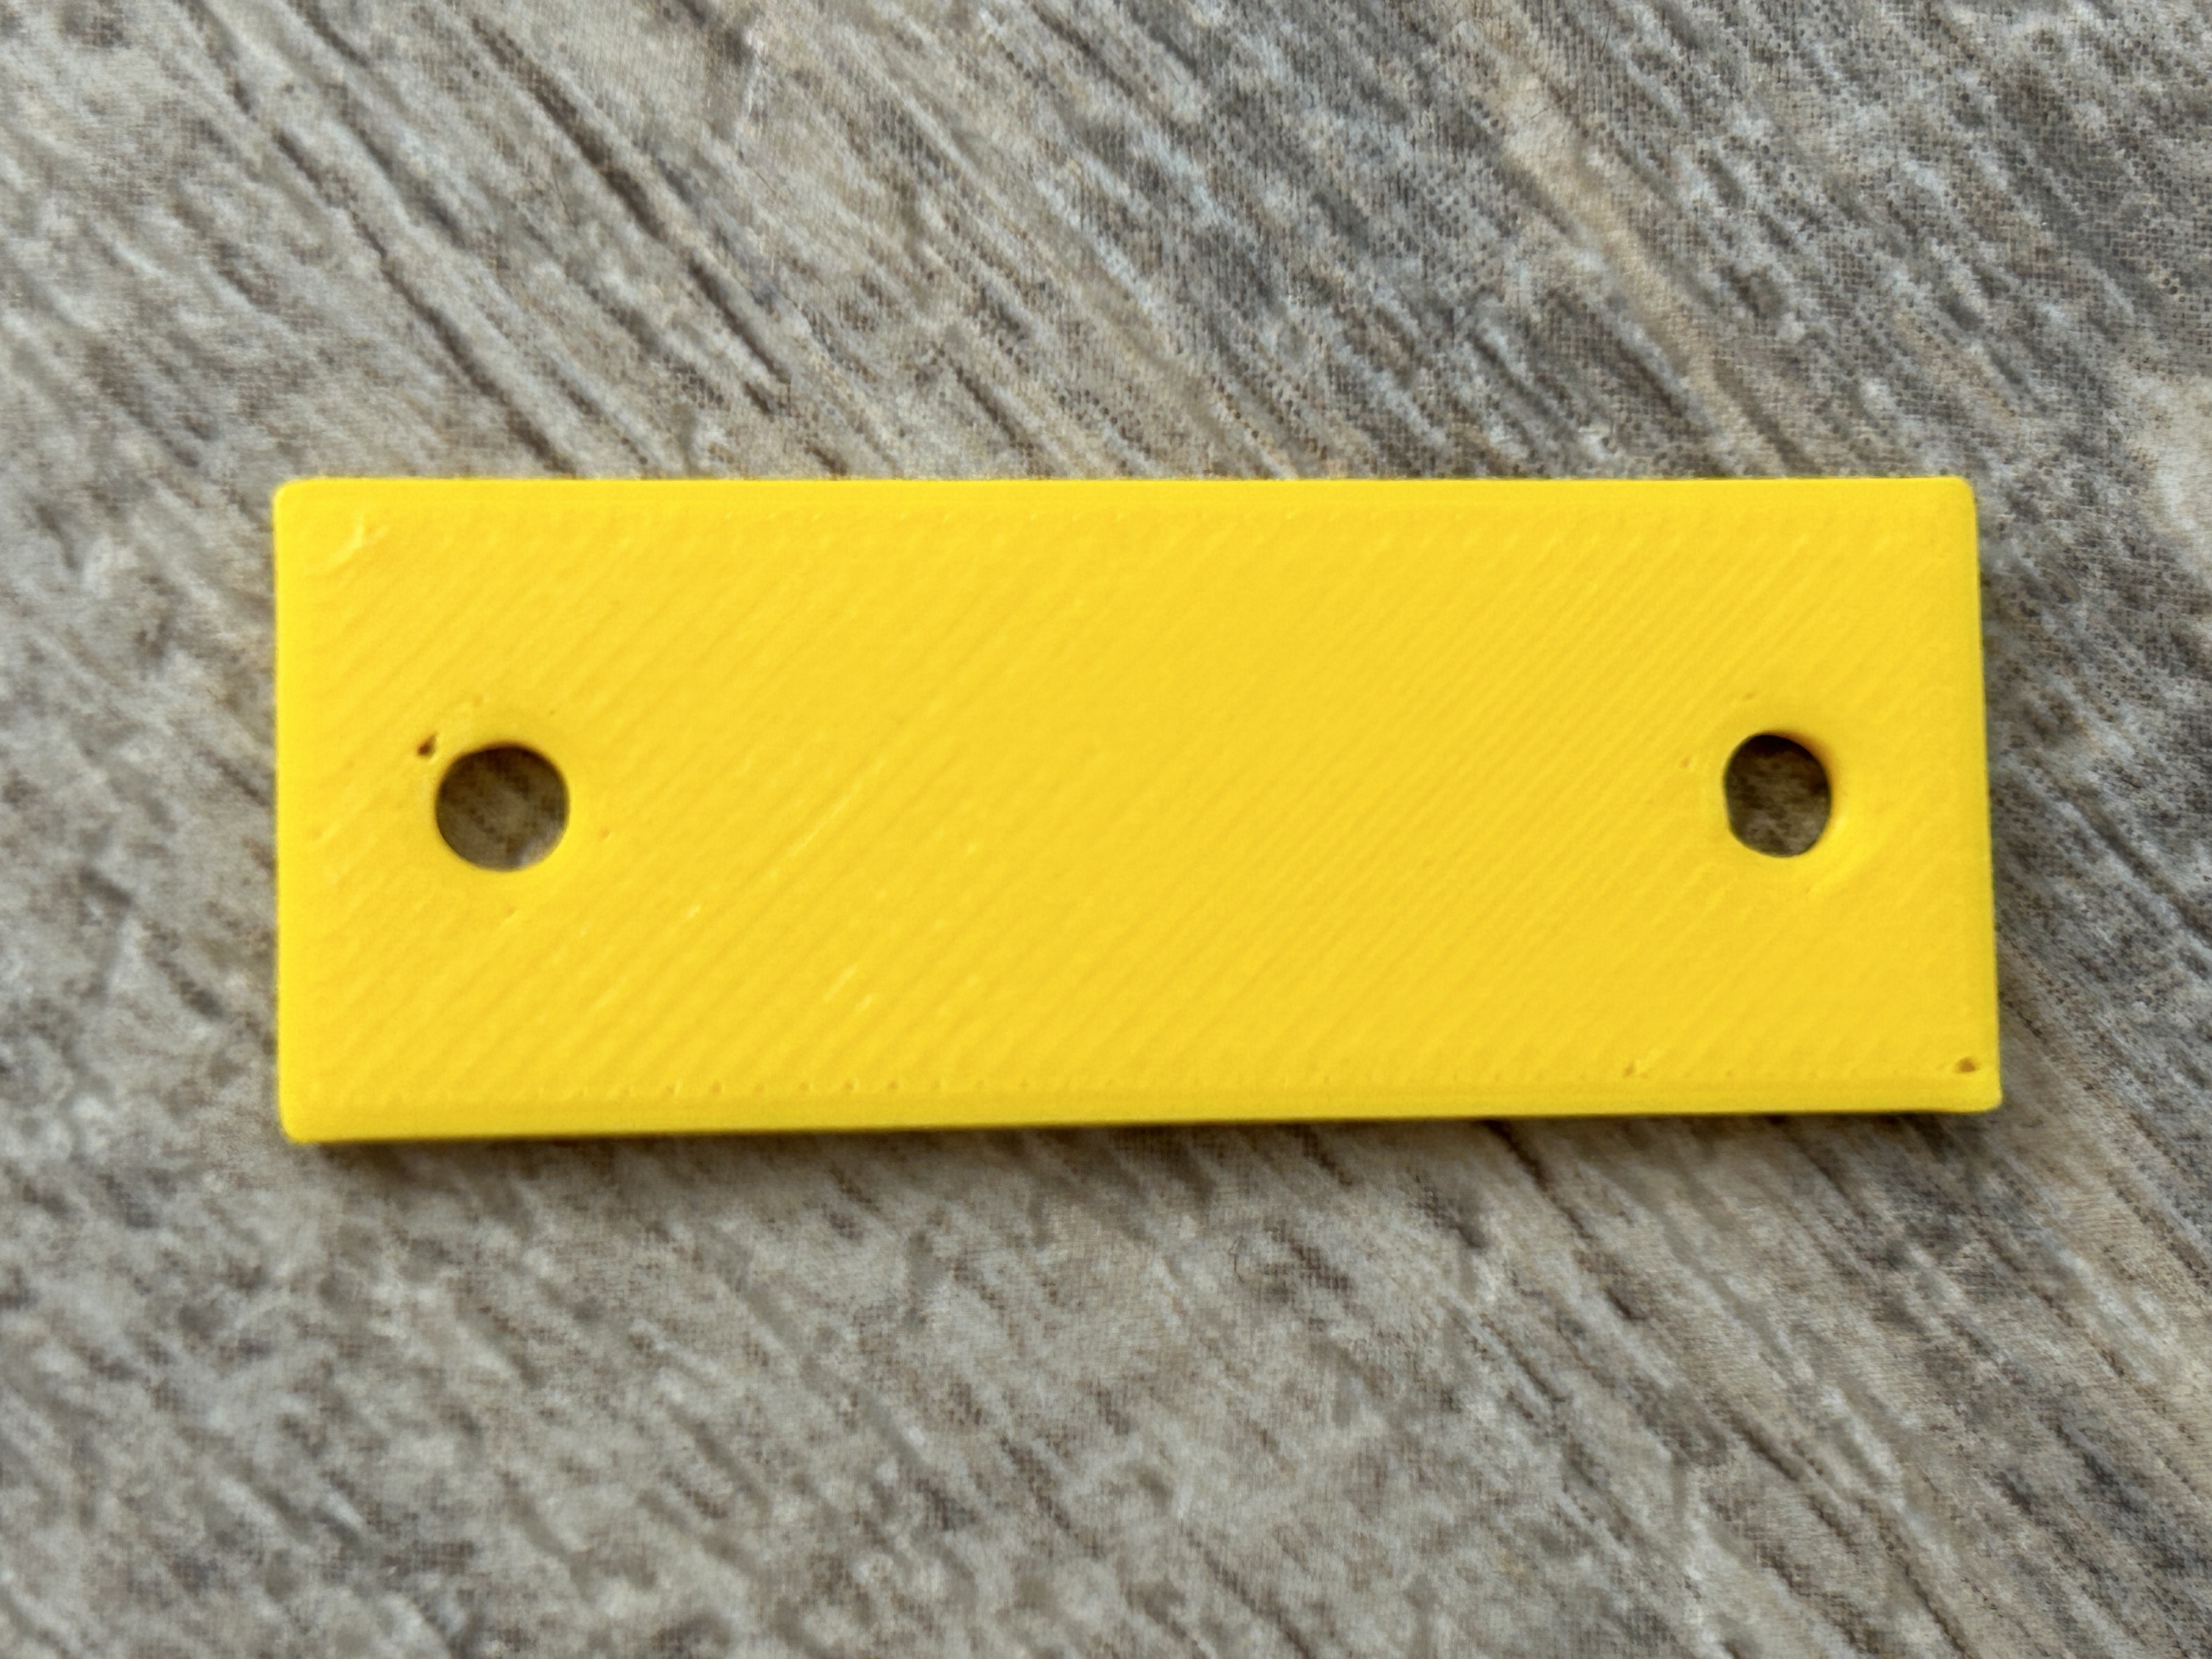
\includegraphics[height=4 cm]{texs/Part1/chapter5/image/res_switch.jpg}
        \end{minipage}
        \caption{Switch Cover}
        \label{fig:printed_switch_cover}
    \end{subfigure}
    \begin{subfigure}[c]{0.45\textwidth}
        \begin{minipage}{\textwidth}
            \centering
            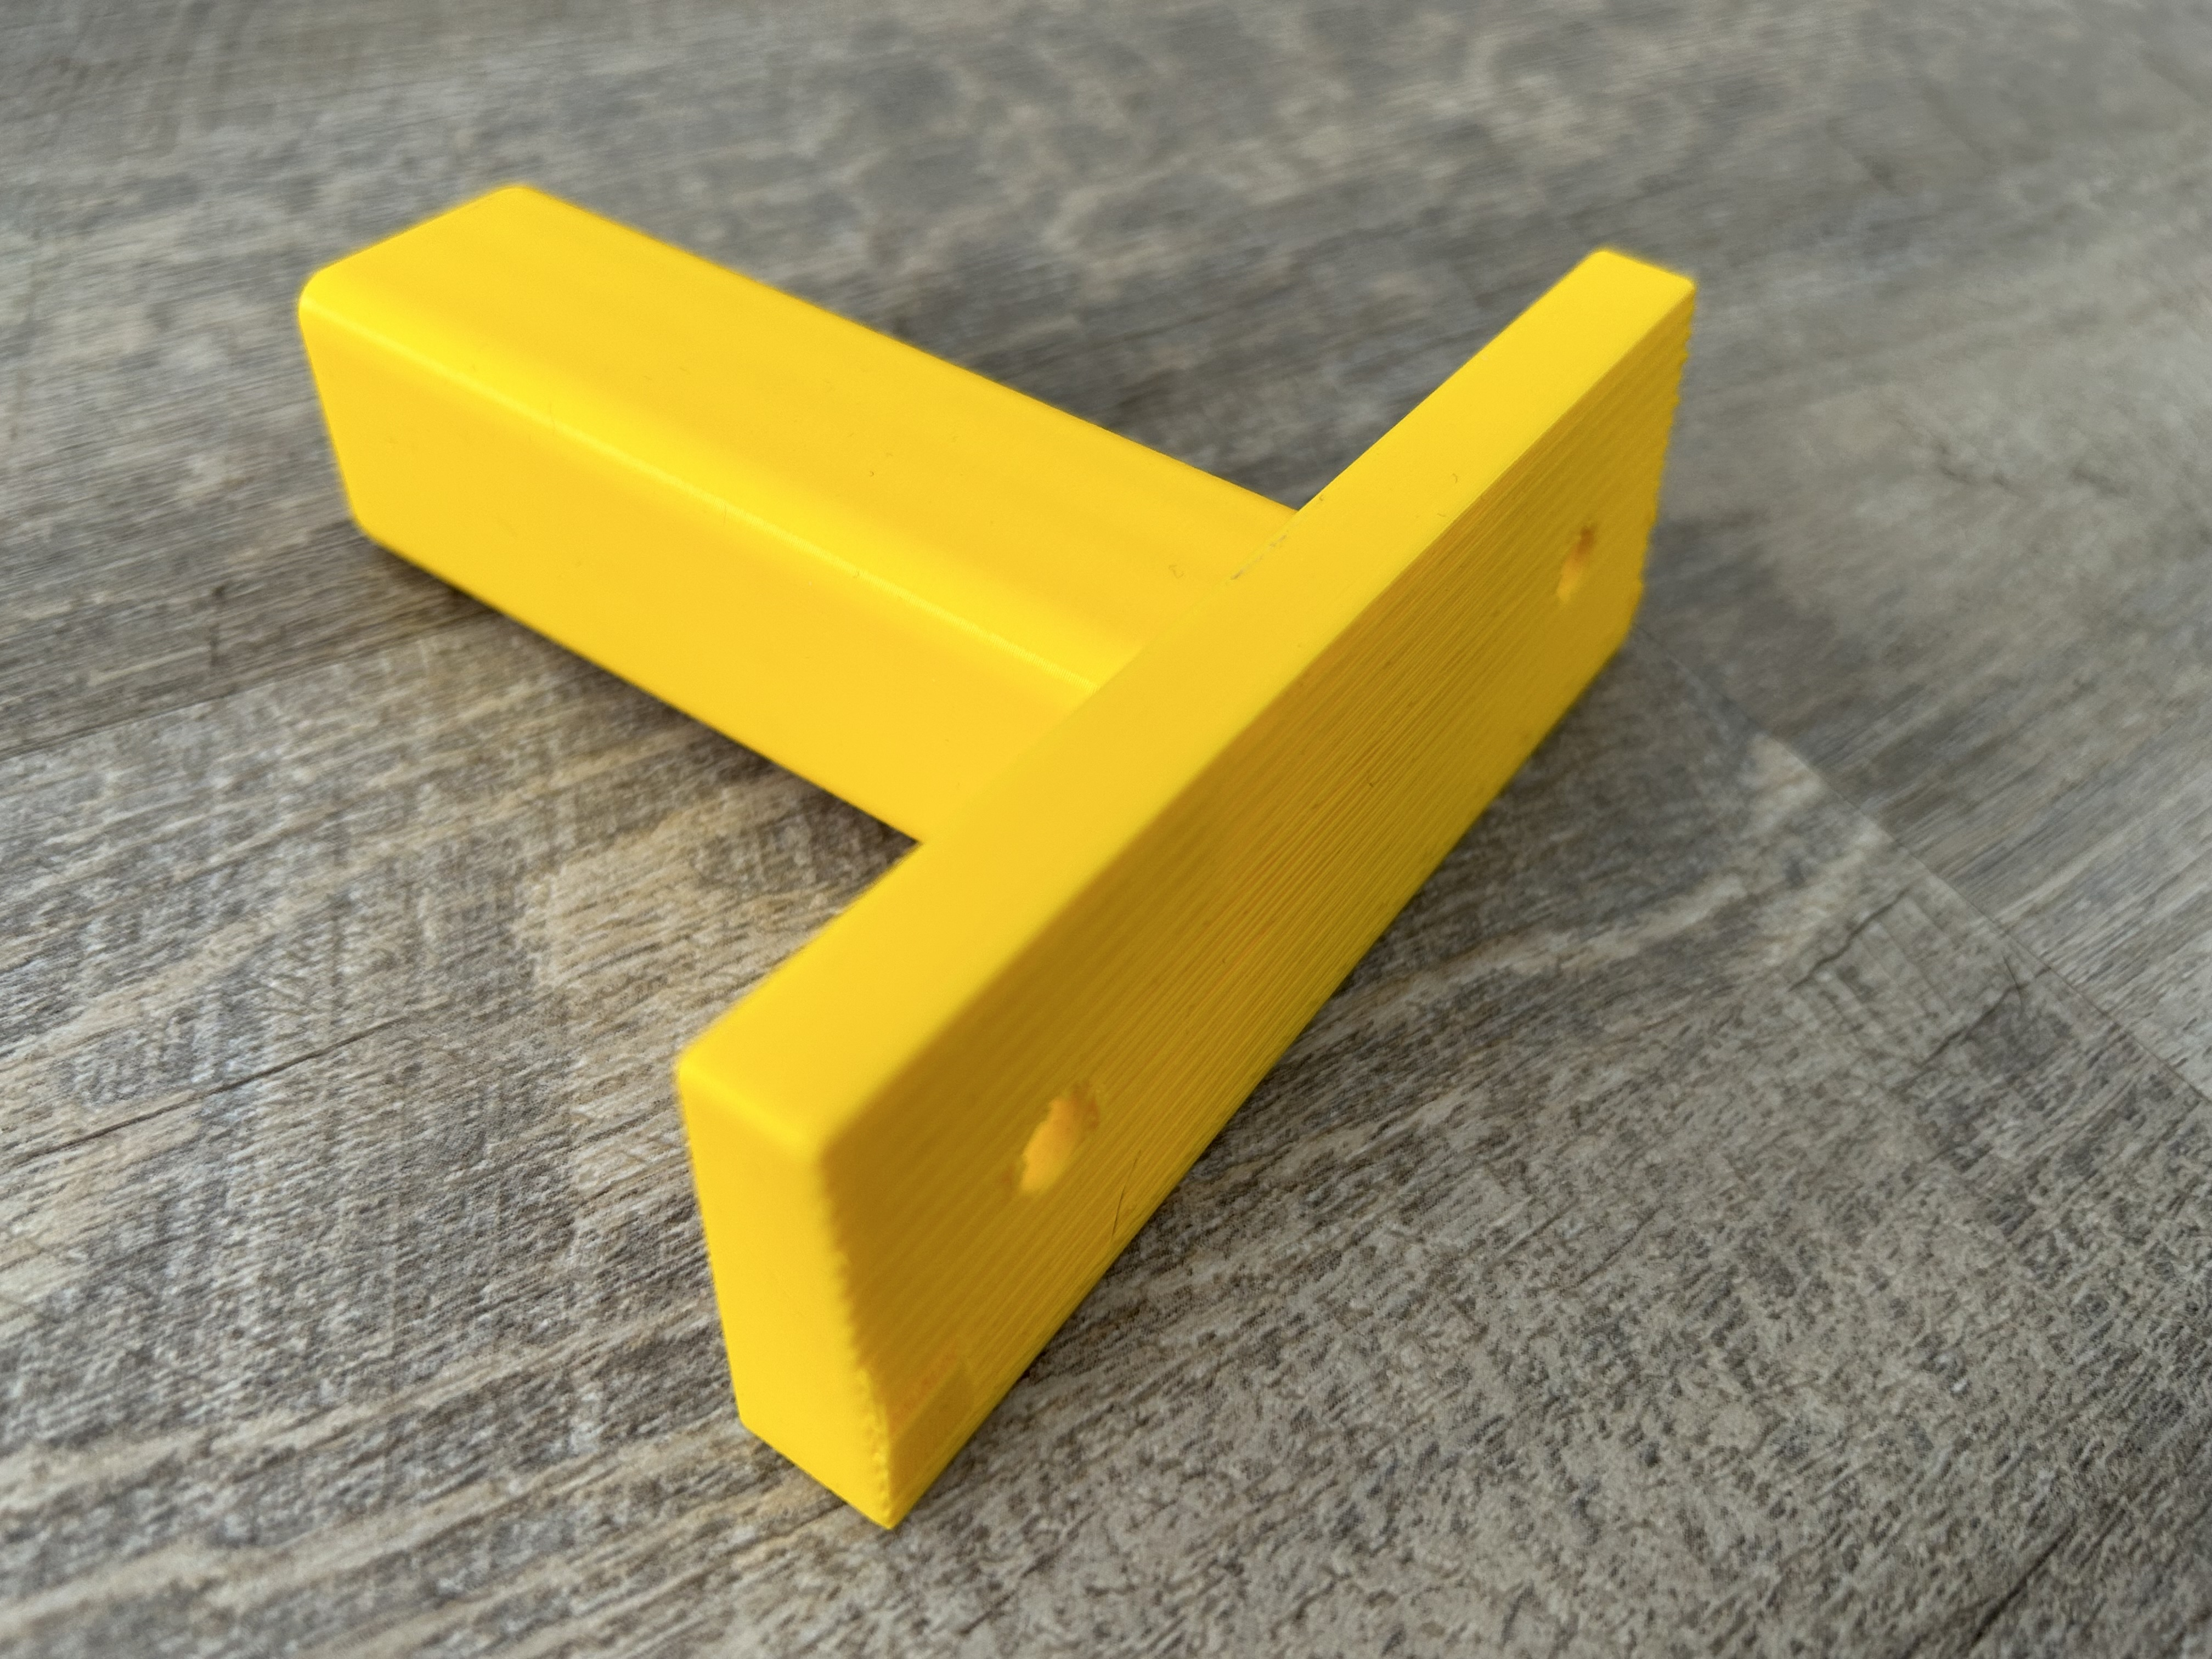
\includegraphics[height=4 cm]{texs/Part1/chapter5/image/res_grip.jpg}
        \end{minipage}
        \caption{Handle Pistol}
        \label{fig:printed_handle_pistol}
    \end{subfigure}
    \caption{Printed Parts}
    \label{fig:printedparts}
\end{figure}

\section{Assembly}
\label{sec:assembly}

The assembly process is done by following the steps below:

\subsubsection{Step 1: Installation of Threaded Inserts}
The brass threaded inserts is installed into the main body by using soldering iron \cite{Hermann23}. To begin, the chosen threaded insert is positioned onto the target material, aligning it with the desired hole. The soldering iron is then heated to an appropriate temperature, typically within the range of 225 to 245 $^{\circ}C$ for PLA material.

As the soldering iron reaches the optimal temperature, it is gently pressed against the top of the threaded insert, transmitting controlled heat directly into the material. This causes the insert to soften and adhere to the surrounding surface, creating a snug fit. Figure \ref{} shows an example of the threaded insert installed into the main body.

\subsubsection{Step 2: Installation of Switch}

Installing a switch to the main body is a straightforward process that requires a few basic materials: the switch itself, a switch cover, two M2.5 nuts, and M2.5 screws. To begin, position the switch inside the designated switch holder (see Figure \ref{fig:switchholder}), ensuring that the button faces outward for easy access.

Next, the switch cover is placed on top of the switch, aligning it with the switch and the corresponding holes in the main body. Once aligned, the M2.5 screws and nuts are used to secure the switch and the switch cover to the main body. Figure \ref{fig:switchinstall} shows the completed installation of the switch.

\begin{figure}
    \centering
    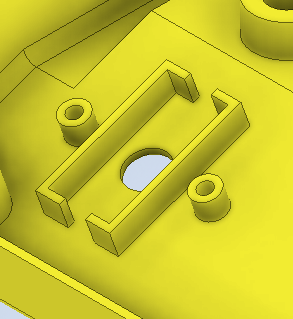
\includegraphics[height=5cm]{texs/Part1/chapter5/image/switchhole.png}
    \caption{The Switch Holder}
    \label{fig:switchholder}
\end{figure}

\begin{figure}
    \centering
    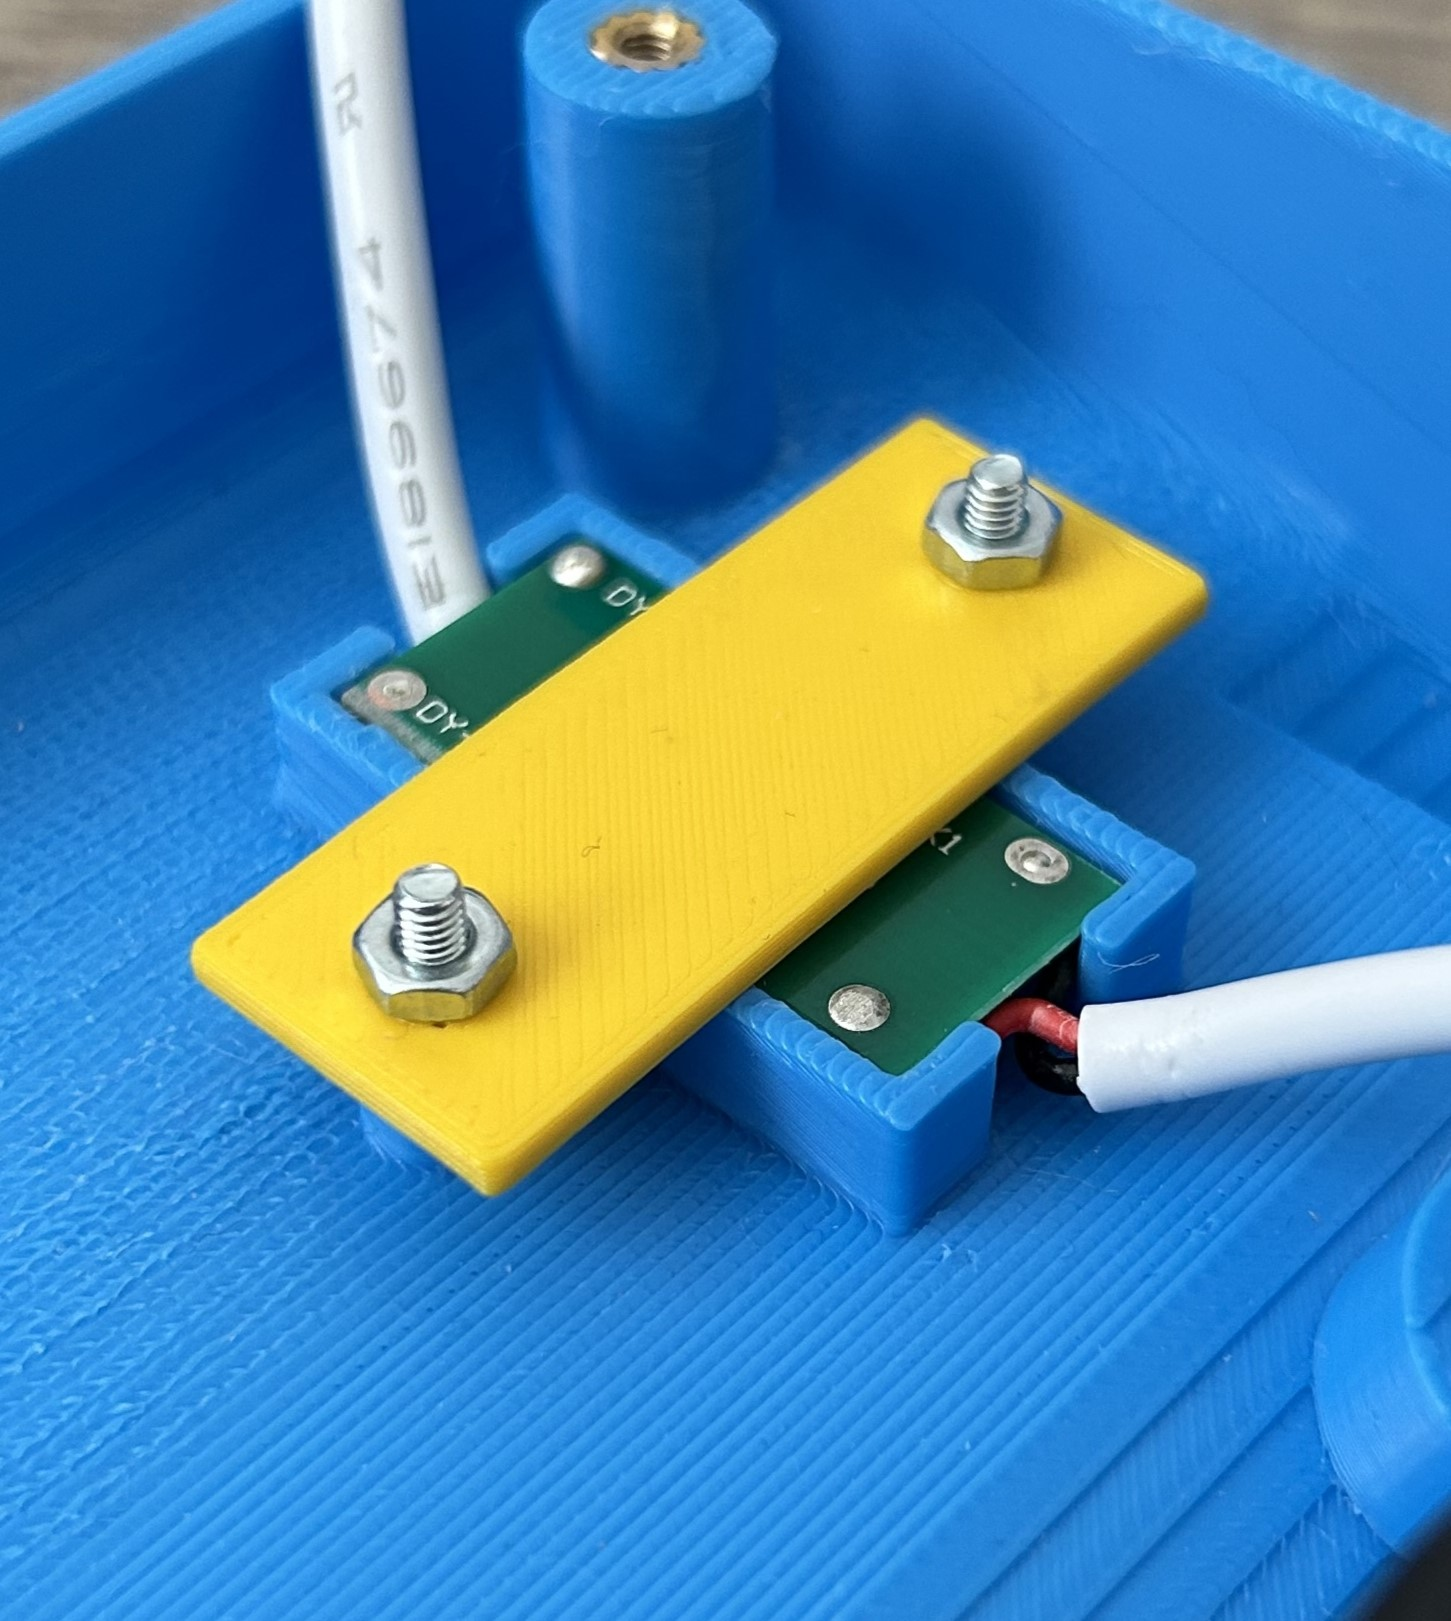
\includegraphics[height=5cm]{texs/Part1/chapter5/image/switchinstall.jpg}
    \caption{The installed switch}
    \label{fig:switchinstall}
\end{figure}

\subsubsection{Step 3: Installation of LAN Port}

This steps begin by locating the slot of the LAN port on the main body, which is located at the right side of the main body (see Figure \ref{fig:lanslot}). The LAN port is then inserted into the slot and secured by using the M3 screws Figure \ref{fig:laninstall} shows the completed installation of the LAN port.

\begin{figure}
    \centering
    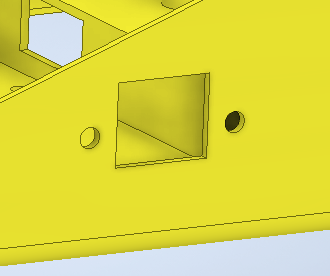
\includegraphics[height=5cm]{texs/Part1/chapter5/image/lanslot.png}
    \caption{The LAN Port Slot}
    \label{fig:lanslot}
\end{figure}

\begin{figure}
    \centering
    \includegraphics[height=5cm]{texs/Part1/chapter5/image/laninstall.jpg}
    \caption{The installed LAN port}
    \label{fig:laninstall}
\end{figure}

\subsubsection{Step 4: Installation of Camera Module}

The camera module is installed to the main body by using the M2 screws. The camera module is placed on the designated slot on the main body (see Figure \ref{fig:cameraslot}). The M2 screws are then used to secure the camera module to the main body. Figure \ref{fig:camerainstall} shows the completed installation of the camera module.

\begin{figure}
    \centering
    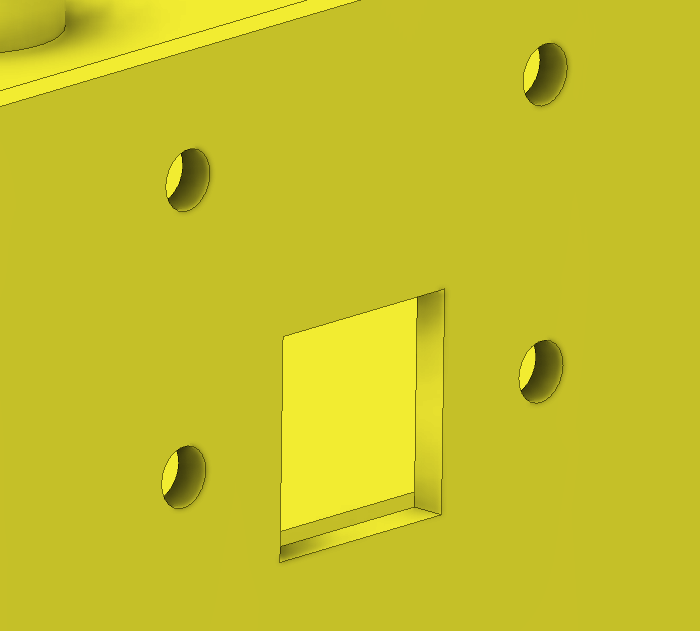
\includegraphics[height=5cm]{texs/Part1/chapter5/image/camslot.png}
    \caption{The Camera Module Slot}
    \label{fig:cameraslot}
\end{figure}

\begin{figure}
    \centering
    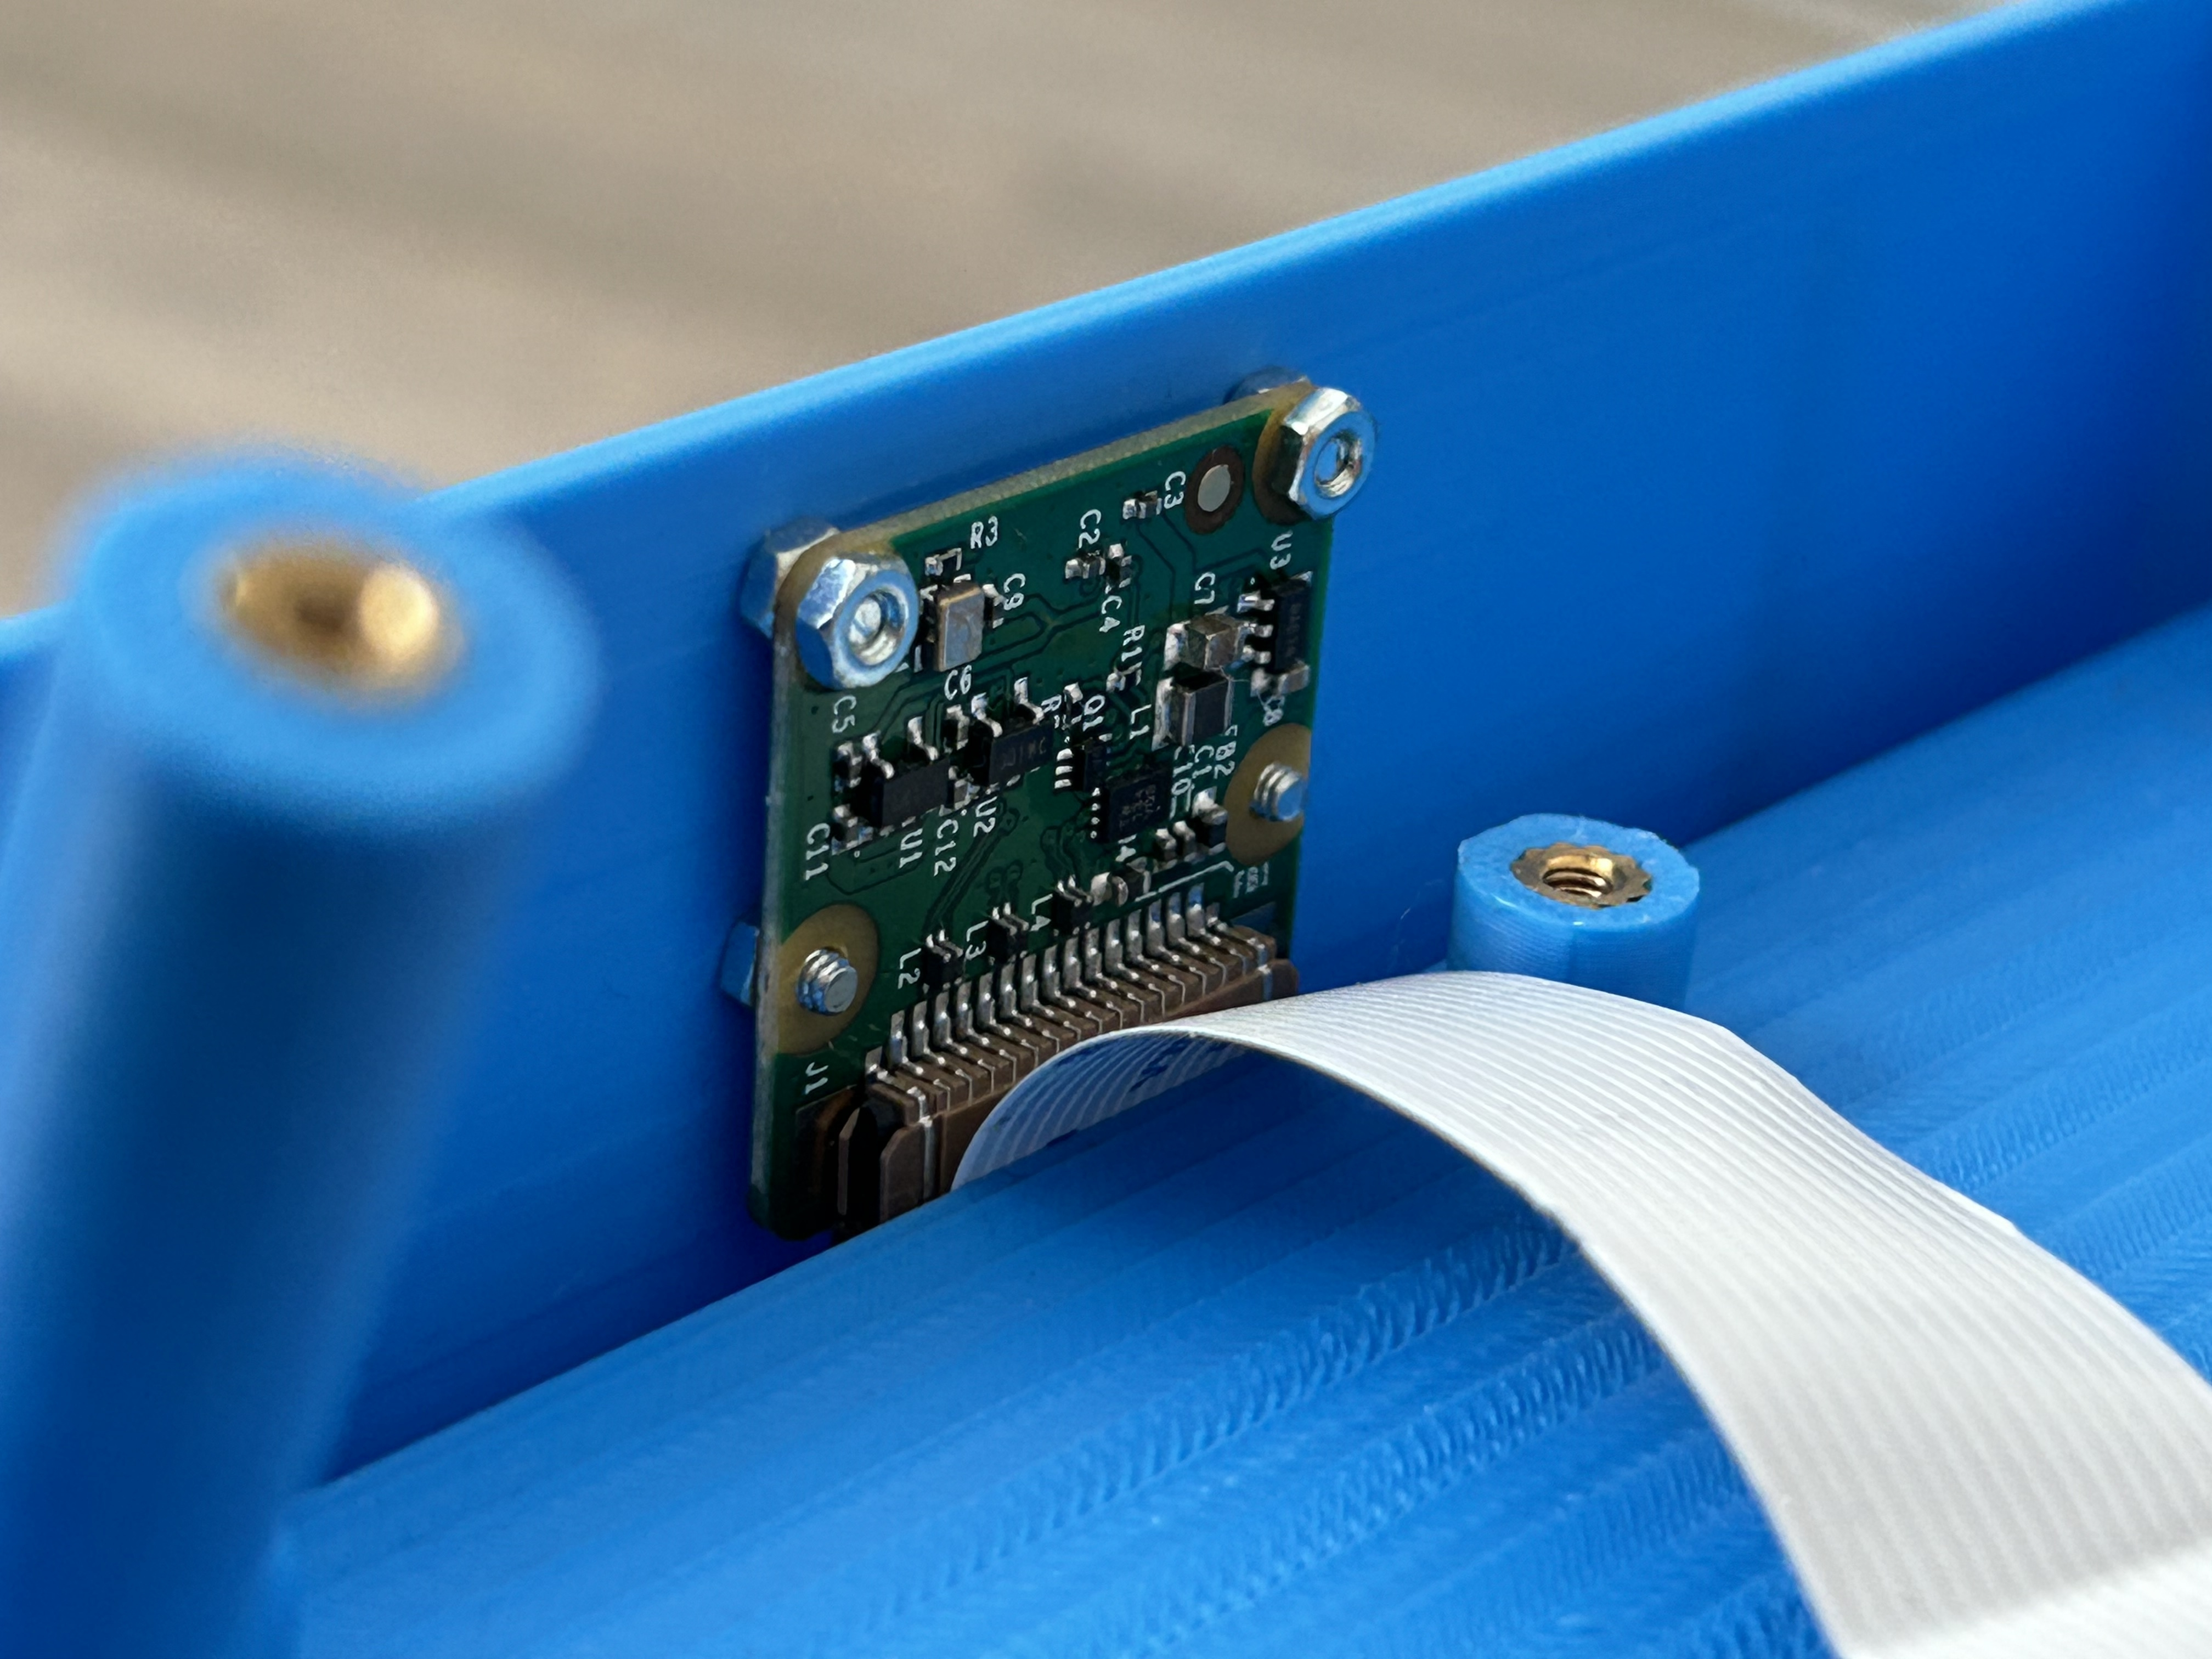
\includegraphics[height=5cm]{texs/Part1/chapter5/image/caminstall.jpg}
    \caption{The installed camera module}
    \label{fig:camerainstall}
\end{figure}

\subsubsection{Step 5: Installation of Battery}
This process begin by placing the battery into the battery holder (see Figure \ref{fig:batteryholder}). Next, the battery is connected the switch via a 90 degree USB-A to USB-C connector.

To secure the battery to the main body, the battery cover is placed on top of the battery and the main body. The M2.5 screws are then used to secure the battery cover to the main body. Figure \ref{fig:batteryinstall} shows the completed installation of the battery.

\begin{figure}
    \centering
    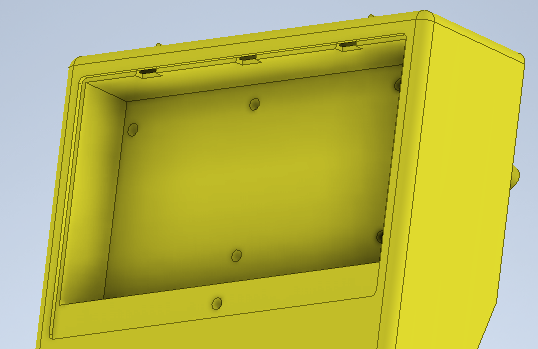
\includegraphics[height=5cm]{texs/Part1/chapter5/image/battslot.png}
    \caption{The Battery Holder}
    \label{fig:batteryholder}
\end{figure}

\begin{figure}[h!]
    \centering
    \begin{subfigure}[c]{0.45\textwidth}
        \begin{minipage}{\textwidth}
            \centering
            \includegraphics[height=5 cm]{texs/Part1/chapter5/image/battinstall1.jpg}
        \end{minipage}
        \caption{Without Battery Cover}
        \label{fig:battery_install_1}
    \end{subfigure}
    \begin{subfigure}[c]{0.45\textwidth}
        \begin{minipage}{\textwidth}
            \centering
            \includegraphics[height=5 cm]{texs/Part1/chapter5/image/battinstall2.jpg}
        \end{minipage}
        \caption{With Battery Cover}
        \label{fig:battery_install_2}
    \end{subfigure}
    \caption{The installed battery}
    \label{fig:batteryinstall}
\end{figure}

\subsubsection{Step 6: Installation of Raspberry Pi}

The Raspberry Pi is installed to the main body by using the M2.5 screws. The Raspberry Pi is placed on the designated slot on the main body (see Figure \ref{fig:raspislot}). The M2.5 screws are then used to secure the Raspberry Pi to the main body.

Next, following connections are made to the Raspberry Pi:


\begin{itemize}
    \item The LAN port is connected to the Raspberry Pi via a LAN cable.
    \item The camera module is connected to the Raspberry Pi via a ribbon cable.
    \item The switch is connected to the Raspberry Pi via USB-C cable.
\end{itemize}

Figure \ref{fig:raspiinstall} shows the completed installation of the Raspberry Pi.

\begin{figure}
    \centering
    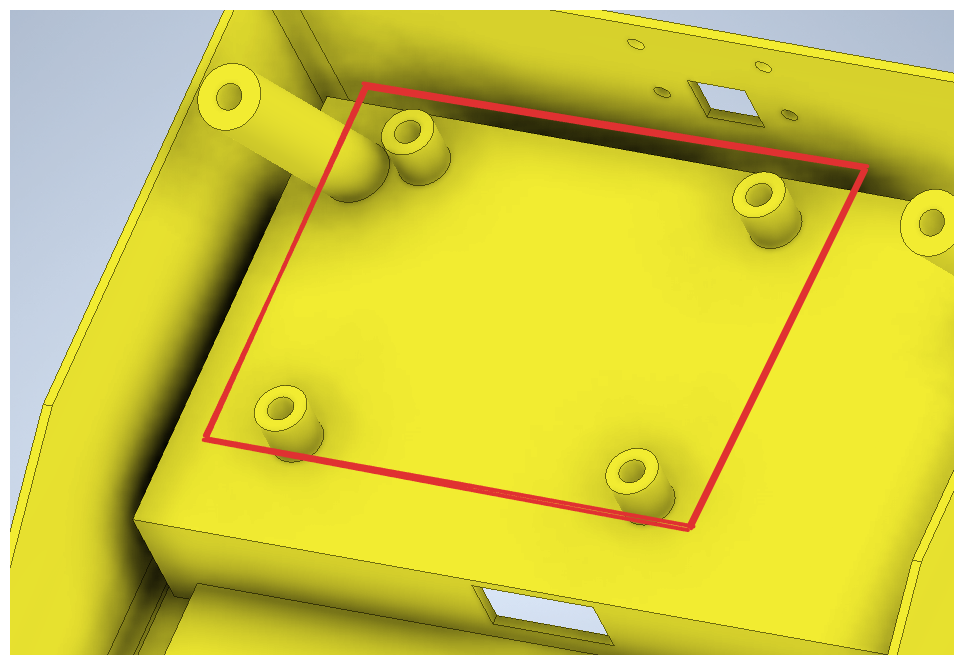
\includegraphics[height=5cm]{texs/Part1/chapter5/image/raspislot.png}
    \caption{The Raspberry Pi Slot}
    \label{fig:raspislot}
\end{figure}

% \begin{figure}
%     \centering
%     \includegraphics[height=5cm]{texs/Part1/chapter5/image/raspiinstall.jpg}
%     \caption{The installed Raspberry Pi}
%     \label{fig:raspiinstall}
% \end{figure}

\subsubsection{Step 7: Installation of Screen and Top Cover}

The final step is to install the screen and the top cover. Begin by placing the screen into the designated slot on the main body (see Figure \ref{fig:screenslot}) and allign the hole on the screen with the hole on the main body. Next, the top cover is placed on top of the main body. The M2.5 screws are then used to secure the top cover to the main body. Figure \ref{fig:screeninstall} shows the completed installation of the screen and the top cover.

\begin{figure}
    \centering
    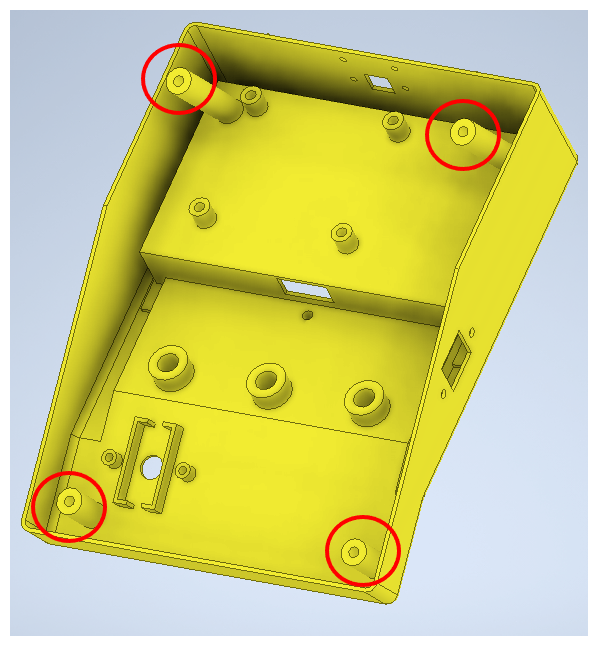
\includegraphics[height=5cm]{texs/Part1/chapter5/image/screenslot.png}
    \caption{The Screen Slot}
    \label{fig:screenslot}
\end{figure}

% \begin{figure}
%     \centering
%     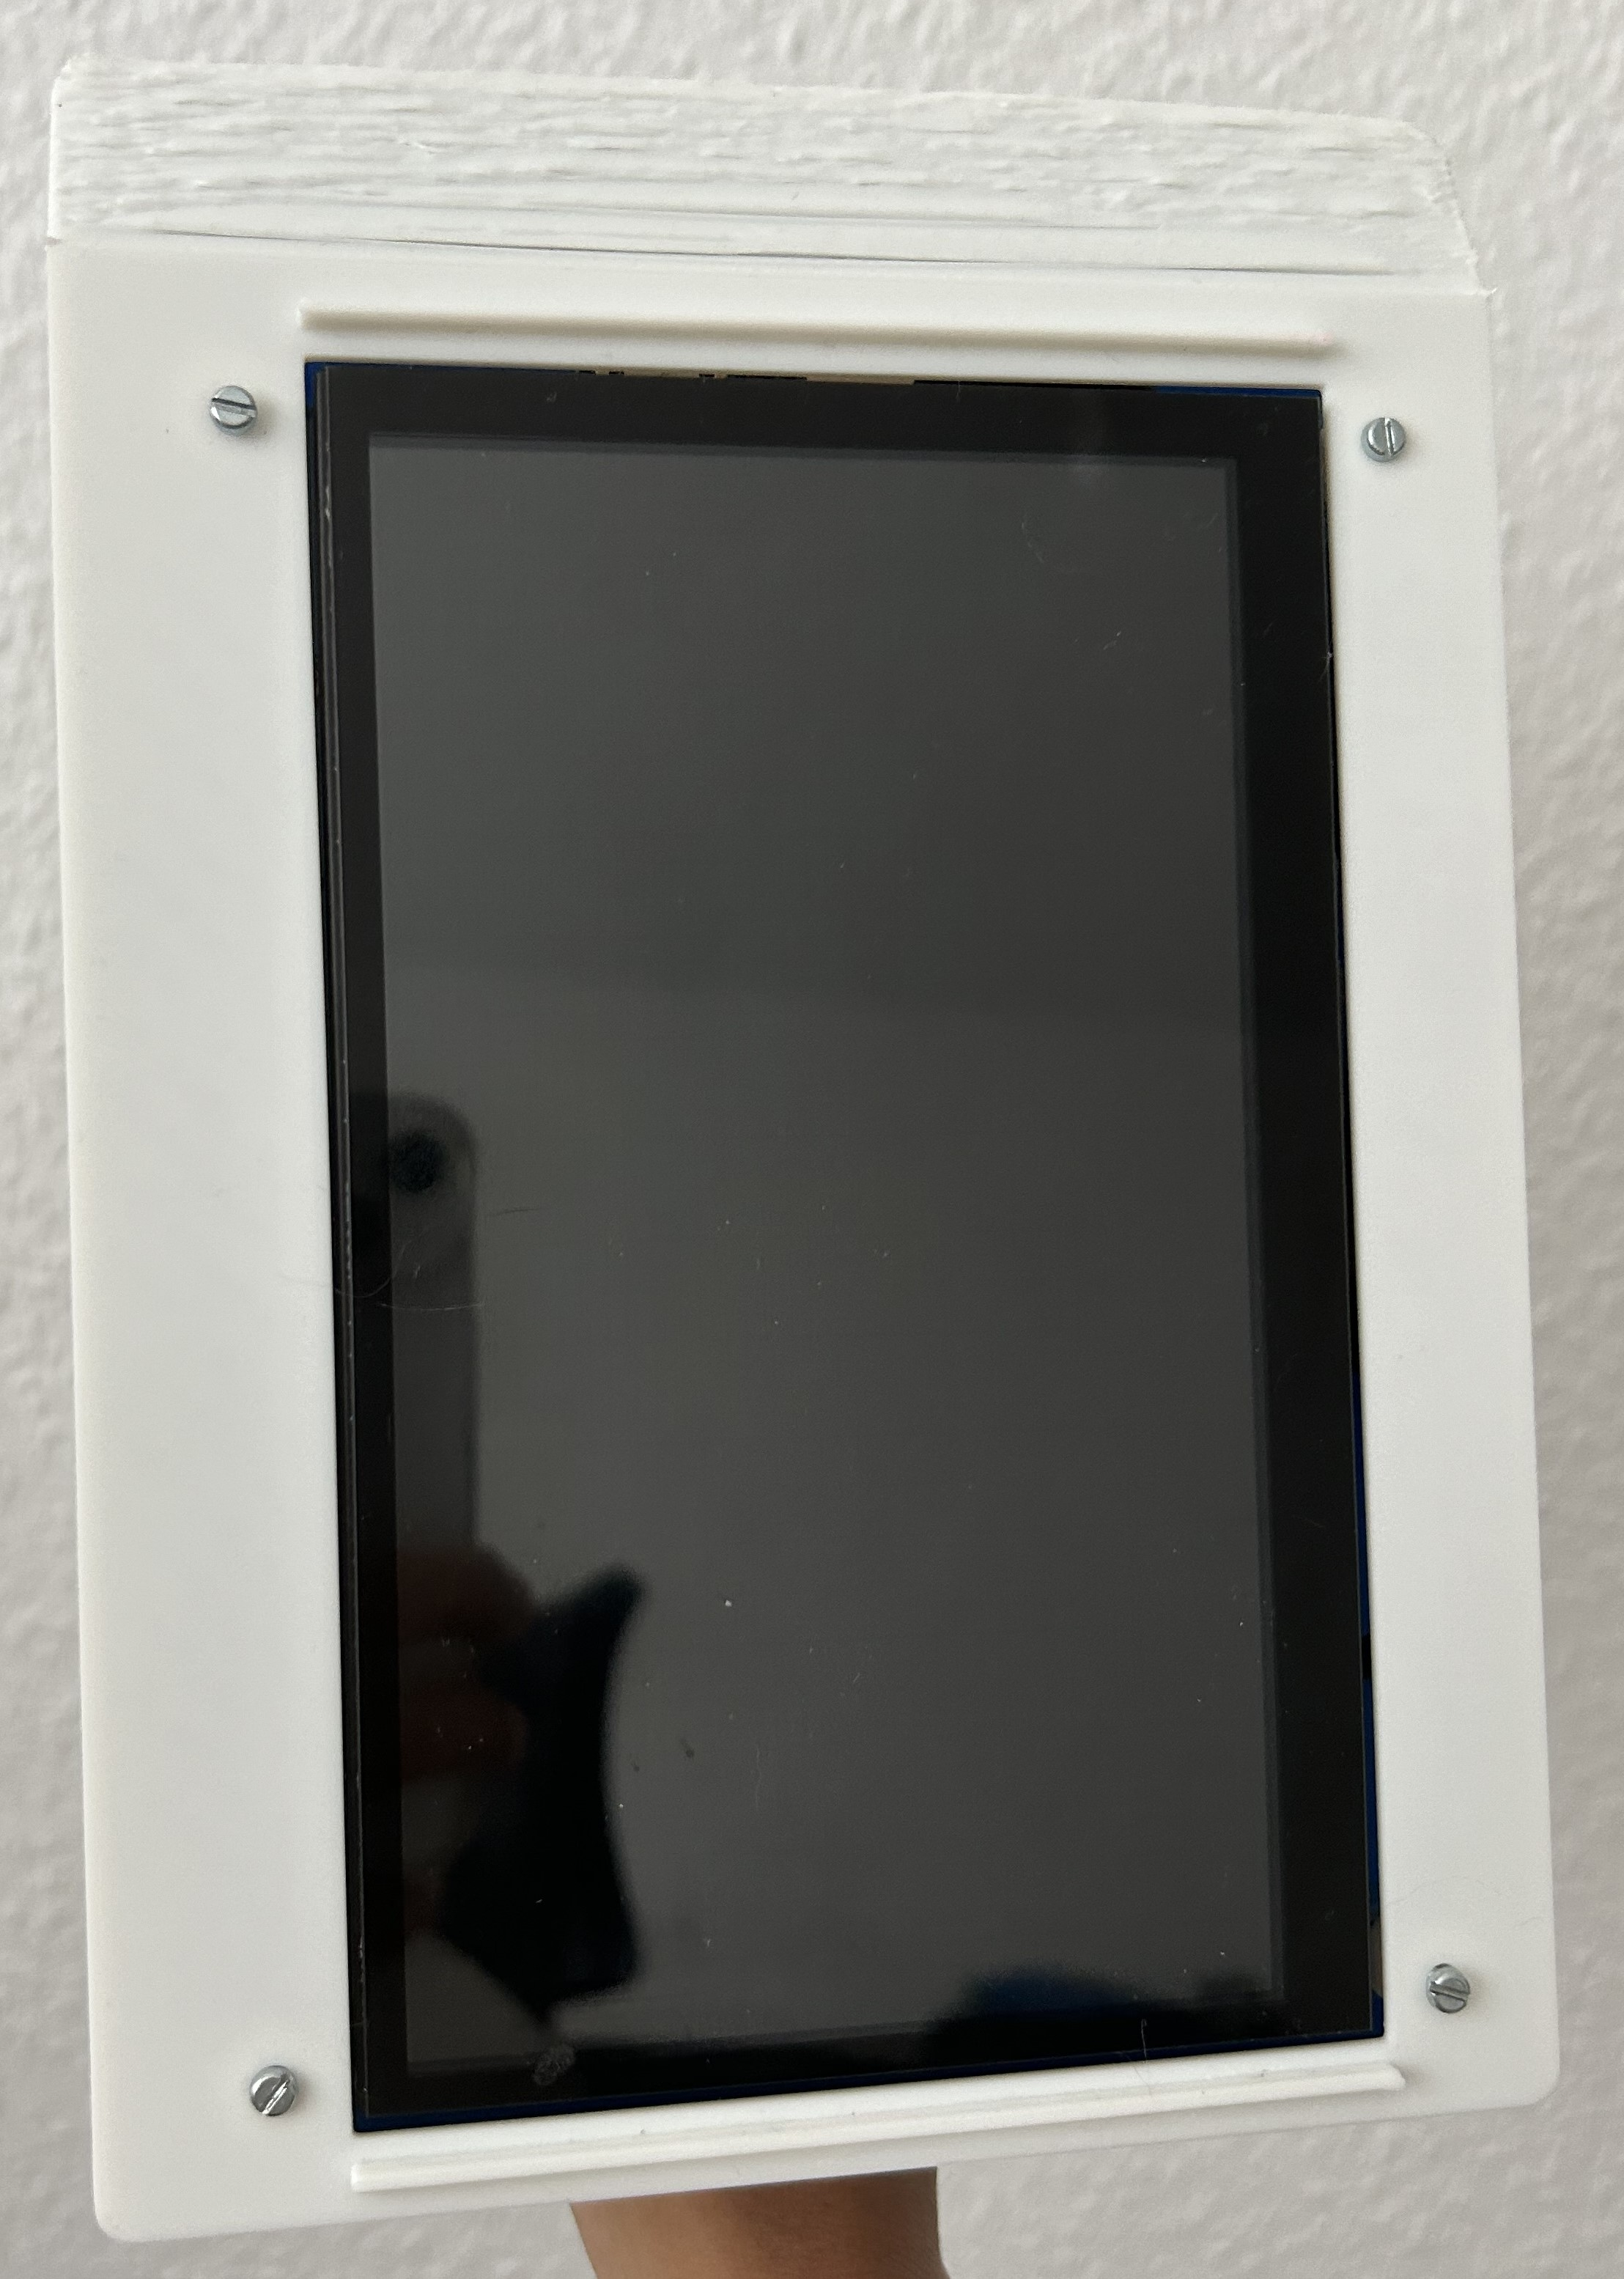
\includegraphics[height=5cm]{texs/Part1/chapter5/image/screeninstall.jpg}
%     \caption{The installed screen and top cover}
%     \label{fig:screeninstall}
% \end{figure}

\section{Final Product}
\label{sec:finalproduct}

Figure \ref{fig:finalproduct} shows the final product. The total cost of building the product including the cost of printing and all of the materials is shown in Table \ref{tab:totalcost}.


\section{Conclusion}